\section{Contribution (2 pages)}

Our approach is based on emergent property estimation techniques \cite{hackenberg2012towards} and uses a model-based approach for validating requirements in early phases of development proposed in \cite{hackenberg2014rapid}, relying on partial system models to ease modeling effort. An adaption to the ITS domain of this modeling technique was proposed in \cite{ascher2014early}, facilitating the formulation of multi-objective traffic flows as an optimal control problem consisting of state variables, control variables, constraints and objectives. The approach employs a generic solver for system behavior estimation, which utilizes stochastic optimization techniques.

In this work, we propose an component-based approach for the exploration and evaluation of future transportation scenarios. Transportation scenarios are considered with respect to the power grid and traffic network. The approach enables the formulation of transportation scenarios through different parameters. Scenarios are defined by objectives, situations and infrastructures representing the defining model parameters. An overview of this approach is shown in Figure~\ref{fig:approach}. 

\textit{Objectives} represent operational costs of different components, such as the traffic network and the power grid. 

\textit{Situations} describe dynamic behavior such as profiles of individual traffic participants and loads on the power grid (i.e. production and consumption). 

\textit{Infrastructures} represent the static structure and landscape of the contained power grid and traffic network. 

Model definition is aided by a composite model architecture fitted to transportation scenario modeling seen in Figure~\ref{fig:model}. On it's highest level, the model architecture is represented by the system model, which contains separate models for the traffic and the power system. The traffic model represents the traffic system, in which individual cars within the traffic infrastructure are contained. Similarly, the power model represents the power system, which is comprised by different energy producing or energy consuming power devices, such as solar panels, energy storages and charging stations. Furthermore, the power system includes the electricity infrastructure, such as low-voltage nets and medium-voltage nets. Model components have a set of input and output ports, which represent observations about specific state variables. Directed connections between ports allow the modeling of interactivity between different components.

After scenario formulation, the approaches enables exploring and identifying the interactions between model parameters. [to be continued]

The main contributions of this paper are:

\begin{enumerate}
	\item Description of a lightweight approach for modeling and exploring dynamics of future
	transportation scenarios based on objectives, situations and infrastructures
	\item Demonstration of the approach using a basic scenario employing a basic traffic network and power grid infrastructure
	and resulting interactions with electric vehicles
\end{enumerate}

\begin{figure}[t!]
	\centering
	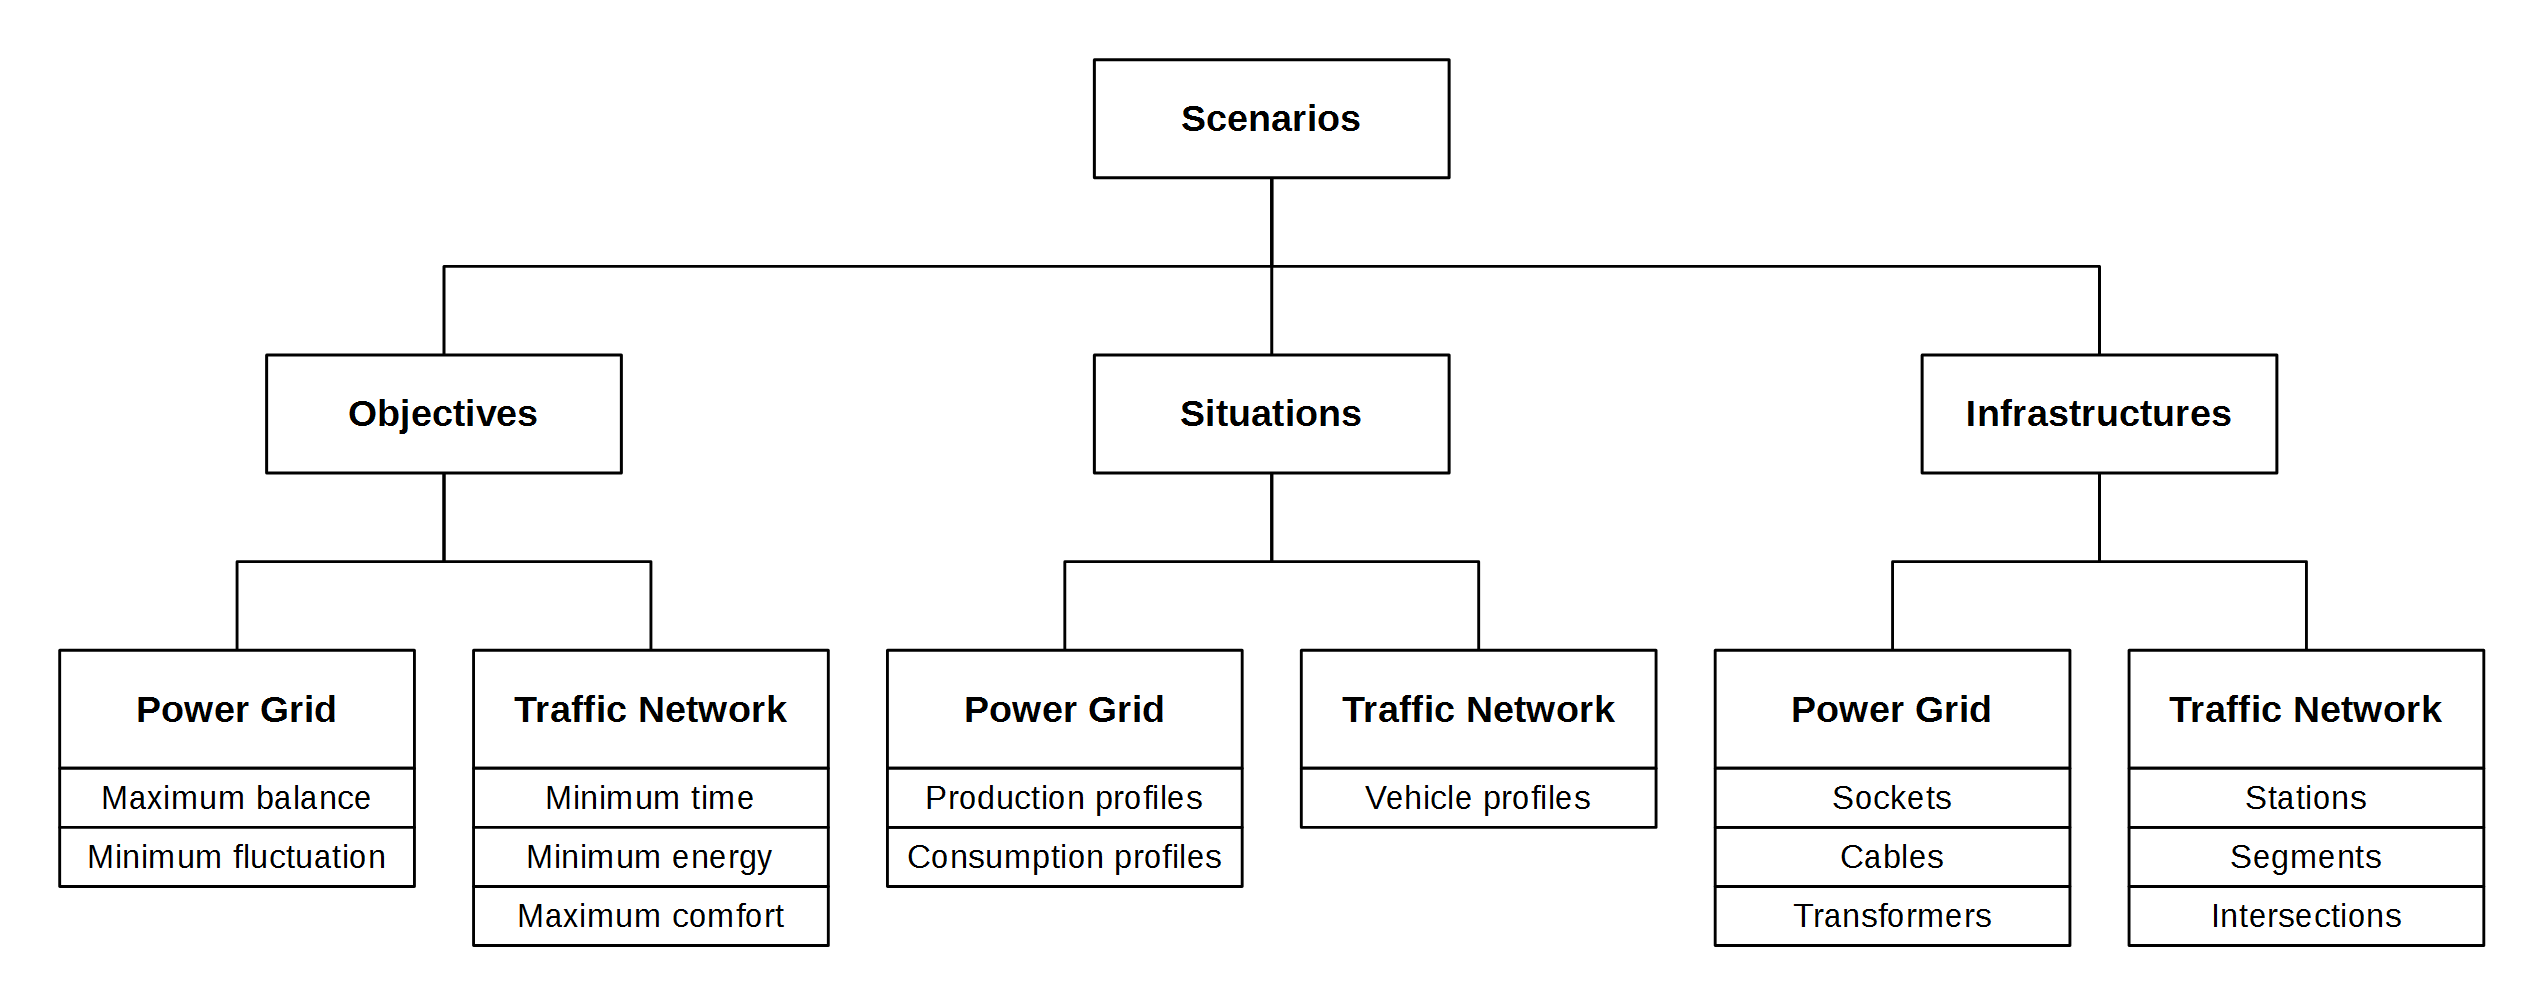
\includegraphics[width=1\columnwidth]{../gfx/approach.png}
	\caption{Overview of transportation scenario modeling including objective, situation and infrastructure parameters for the power grid and the traffic network.}
	\label{fig:approach}
\end{figure}

Subsequently we describe the different components of the model architecture based on their state variables, control variables, constraints and objectives. 

\begin{figure}[t!]
	\centering
	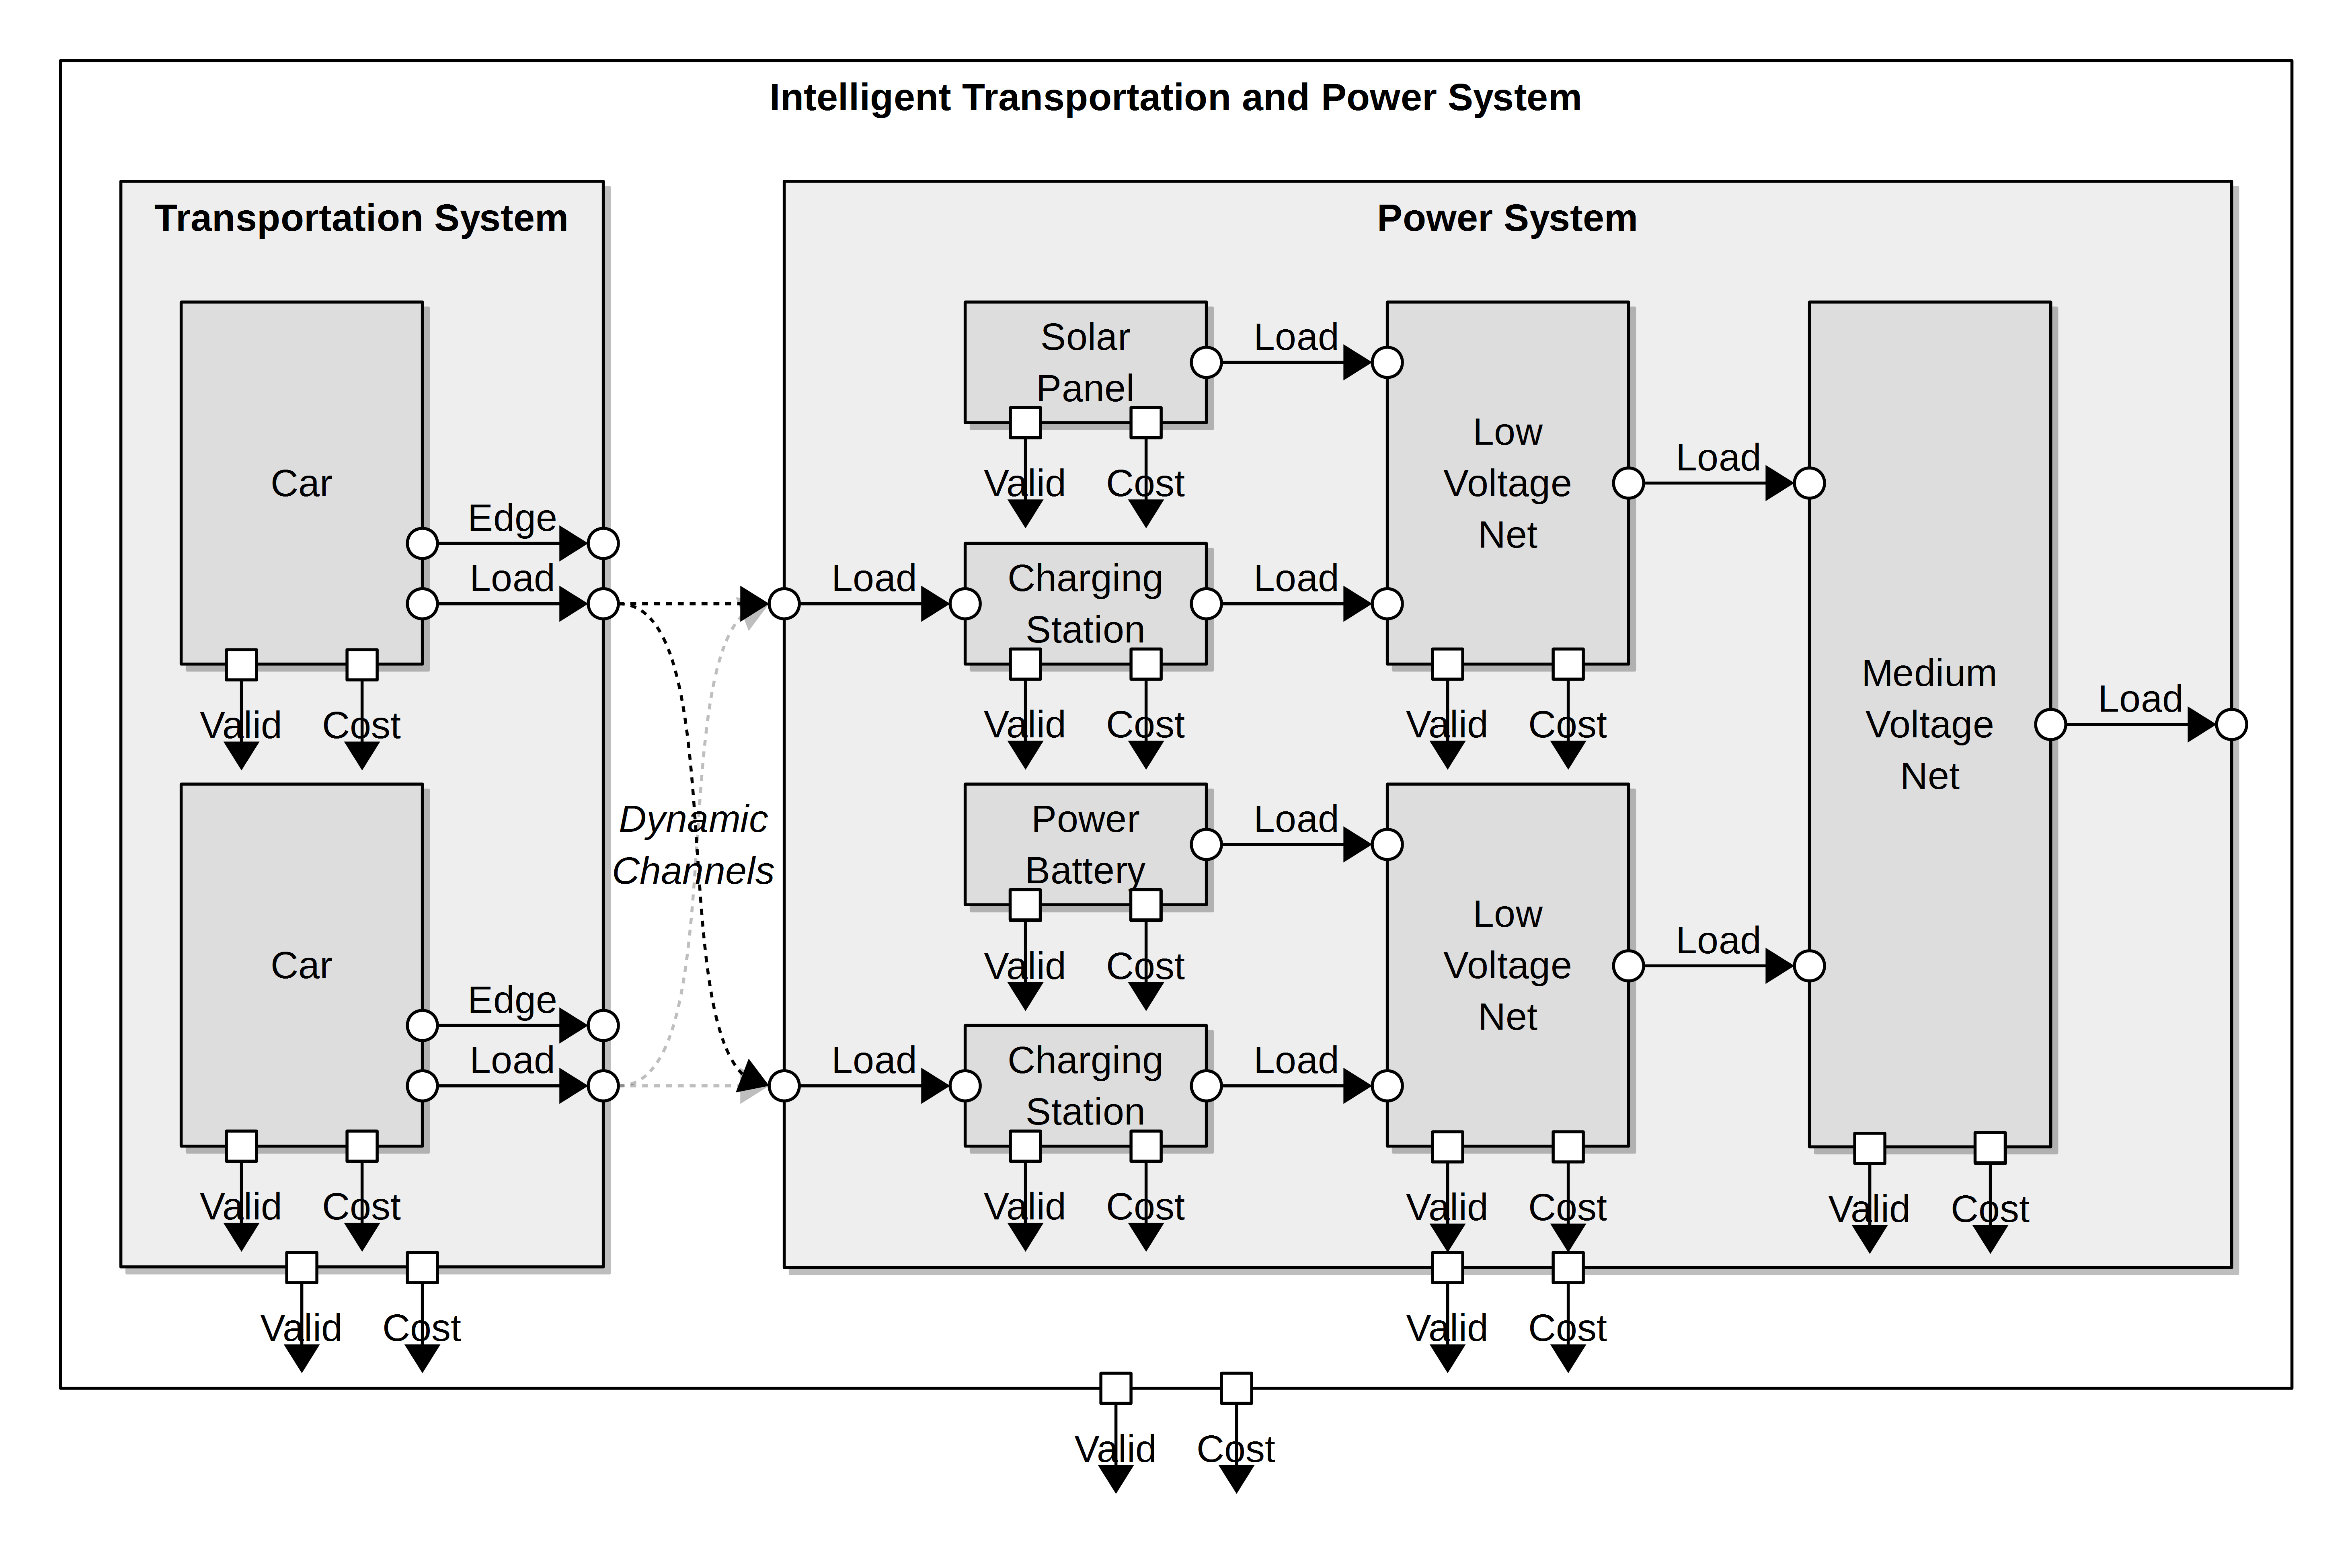
\includegraphics[width=0.925\columnwidth]{../gfx/model.png}
	\caption{Overview of model architecture fitted to transportation scenario modeling}
	\label{fig:model}
\end{figure}

\subsection{System Model}

E.g. system model consists of (1) Transportation System and (2) Power System.


\subsection{Traffic Model}

TBD

\subsubsection{Traffic System}

TBD

\subsubsection{Car}

TBD

\subsection{Power Model}

TBD

\subsubsection{Power System}

TBD

\subsubsection{Net}

TBD

\subsubsection{Solar}

TBD

\subsubsection{Storage}

TBD

\subsubsection{Charging Station}

TBD

\subsection{Scenario Modeling}

Parameters

TBD